\documentclass[border=10pt]{standalone}

\usepackage{tikz}
\usepackage{tikzsymbols}
\usetikzlibrary{calc,patterns,shapes.geometric}

\def\centerarc[#1](#2)(#3:#4:#5){\draw[#1] ($(#2)+({#5*cos(#3)},{#5*sin(#3)})$) arc (#3:#4:#5);}

\begin{document}
	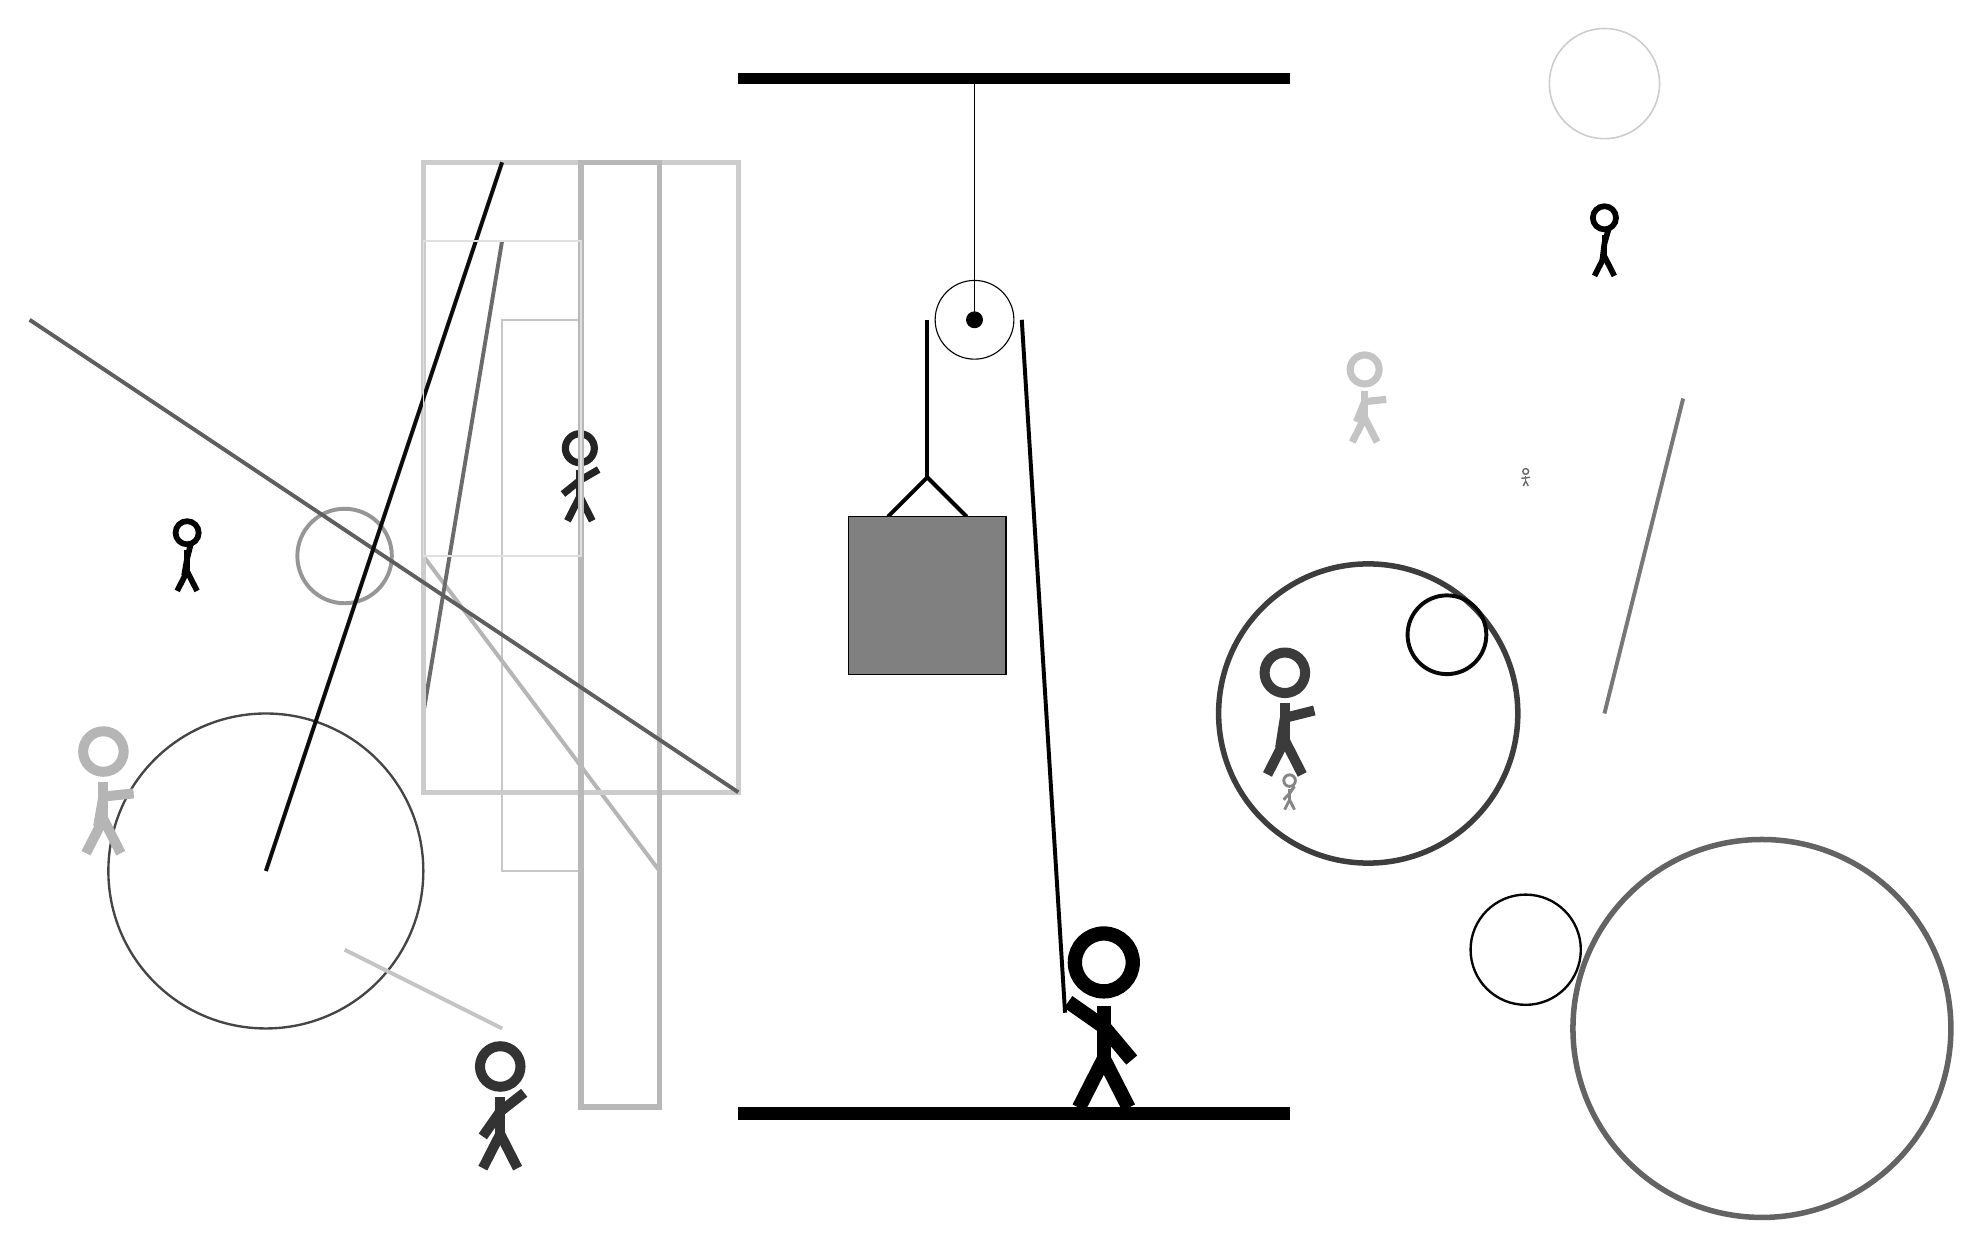
\begin{tikzpicture}
		%%%%% START %%%%%
		
		\draw[fill=black] (-2, 10) rectangle (5, 10.125);
		
		\draw (1, 7) circle (0.5);
		\draw[fill=black] (1, 7) circle (0.1);
		\draw (1, 10) -- (1, 7);
		
		\draw[line width=0.5mm] (-0.1, 4.5) -- (0.4, 5.0) -- (0.9, 4.5);
		\draw[fill=black!50] (-0.6, 4.5) rectangle (1.4, 2.5);
		
		\draw [line width=0.7mm, color=black!61](11, -2) circle (2.4);
		
		\draw[line width=0.3mm, color=black!22] (-4, 7) rectangle (-5, 0);
		\draw[line width=0.5mm, color=black!29](-6, 4) -- (-3, 0);
		\node[line width=0.5mm, color=black!77] at (5, 2) {\Strichmaxerl[7][81][14]};
		
		\draw [line width=0.3mm, color=black!73](-8, 0) circle (2.0);
		\draw[line width=0.5mm, color=black!23](-7, -1) -- (-5, -2);
		
		\draw[line width=0.5mm, color=black!58](-6, 2) -- (-5, 8);
		
		\draw [line width=0.5mm, color=black!41](-7, 4) circle (0.6);
		\draw [line width=0.3mm, color=black!98](8, -1) circle (0.7);
		\draw [line width=0.7mm, color=black!76](6, 2) circle (1.9);
		
		\draw [line width=0.2mm, color=black!20](9, 10) circle (0.7);
		
		\node[line width=0.4mm, color=black!98] at (-9, 4) {\Strichmaxerl[4][80][76]};
		\node[line width=0.2mm, color=black!48] at (5, 1) {\Strichmaxerl[2][46][56]};
		
		\node[line width=0.4mm, color=black!29] at (-10, 1) {\Strichmaxerl[7][80][6]};
		\node[line width=0.3mm, color=black!59] at (8, 5) {\Strichmaxerl[1][5][8]};
		\node[line width=0.3mm, color=black!80] at (-5, -3) {\Strichmaxerl[7][55][38]};
		
		\draw[line width=0.6mm, color=black!20] (-2, 1) rectangle (-6, 9);
		
		\node[line width=0.5mm, color=black!86] at (-4, 5) {\Strichmaxerl[5][39][30]};
		\draw[line width=0.7mm, color=black!28] (-3, 9) rectangle (-4, -3);
		\draw [line width=0.5mm, color=black!97](7, 3) circle (0.5);
		\draw[line width=0.5mm, color=black!53](9, 2) -- (10, 6);
		
		\draw[line width=0.5mm, color=black!63](-2, 1) -- (-11, 7);
		\node[line width=0.2mm, color=black!100] at (9, 8) {\Strichmaxerl[4][83][74]};
		\draw[line width=0.5mm, color=black!95](-5, 9) -- (-8, 0);
		\node[line width=0.5mm, color=black!23] at (6, 6) {\Strichmaxerl[5][68][6]};
		
		\draw[line width=0.2mm, color=black!12] (-4, 8) rectangle (-6, 4);
		
		\draw[line width=0.5mm] (0.4, 7) -- (0.4, 5.0);
		\centerarc[line width=0.5mm](1, 7)(0:180:0.6);
		\draw[line width=0.5mm](1.6, 7) -- (2.15, -1.8);
		
		\node at (2.6, -1.9) {\Strichmaxerl[10][-35][-50]};
		
		\draw[fill=black] (-2, -3) rectangle (5, -3.15);
		
		%%%%% END %%%%%
	\end{tikzpicture}
\end{document}